\documentclass{beamer}
\usepackage{graphicx}
\usepackage{hyperref}
\usepackage[sorting=none]{biblatex}
\usepackage[font=small,skip=0pt]{caption}
\bibliography{refs}
\usepackage{tikz}
\renewcommand{\footnotesize}{\fontsize{8pt}{8pt}\selectfont}
\usetheme{Madrid}
\usecolortheme{beaver}
\titlegraphic{
\includegraphics[width=2.5cm]{logo.png}}
\title[High Harmonic Generation]{High Harmonic Generation in Laser Plasma Interaction}
\date{}
\institute[IIT Delhi]{\large Indian Institute of Technology, Delhi}
\author[]{Kulwinder Kaur (2021PHS7190)\\ Harikesh Kushwaha (2021PHS7181)\\[3mm]Adviser: Prof. Vikrant Saxena}
\vspace{0cm}
\begin{document}
\maketitle

\begin{frame}{Introduction}
    \frametitle{Introduction}
    \small
    Interaction of light with matter at ultra high light intensity gives access to novel physical regimes which are barely, if at all, explored in lab.
    \begin{itemize}
        \item Intensity of $10^{23} \; W/cm^{-2}$ has been reached experimentally.\footnote{\textit{Henri Vincenti} 10.1103/physrevlett.123.105001}
        \item QED at $I = 10^{25}W/cm^{-2}$. Schwinger field at $I = 10^{29}W/cm^{-2}$.\footnote{\textit{Jin Woo Yoon et al} 10.1364/OPTICA.420520}
        \item Plasma is overdense if $\omega<\omega_p$.
        \item Harmonics are generated by interaction of laser with overdense plasma.\footnote{\textit{R. Lichters et al} 10 . 1063 / 1 . 871619}
    \end{itemize}
    \begin{minipage}[h]{0.48\linewidth}
        \centering
        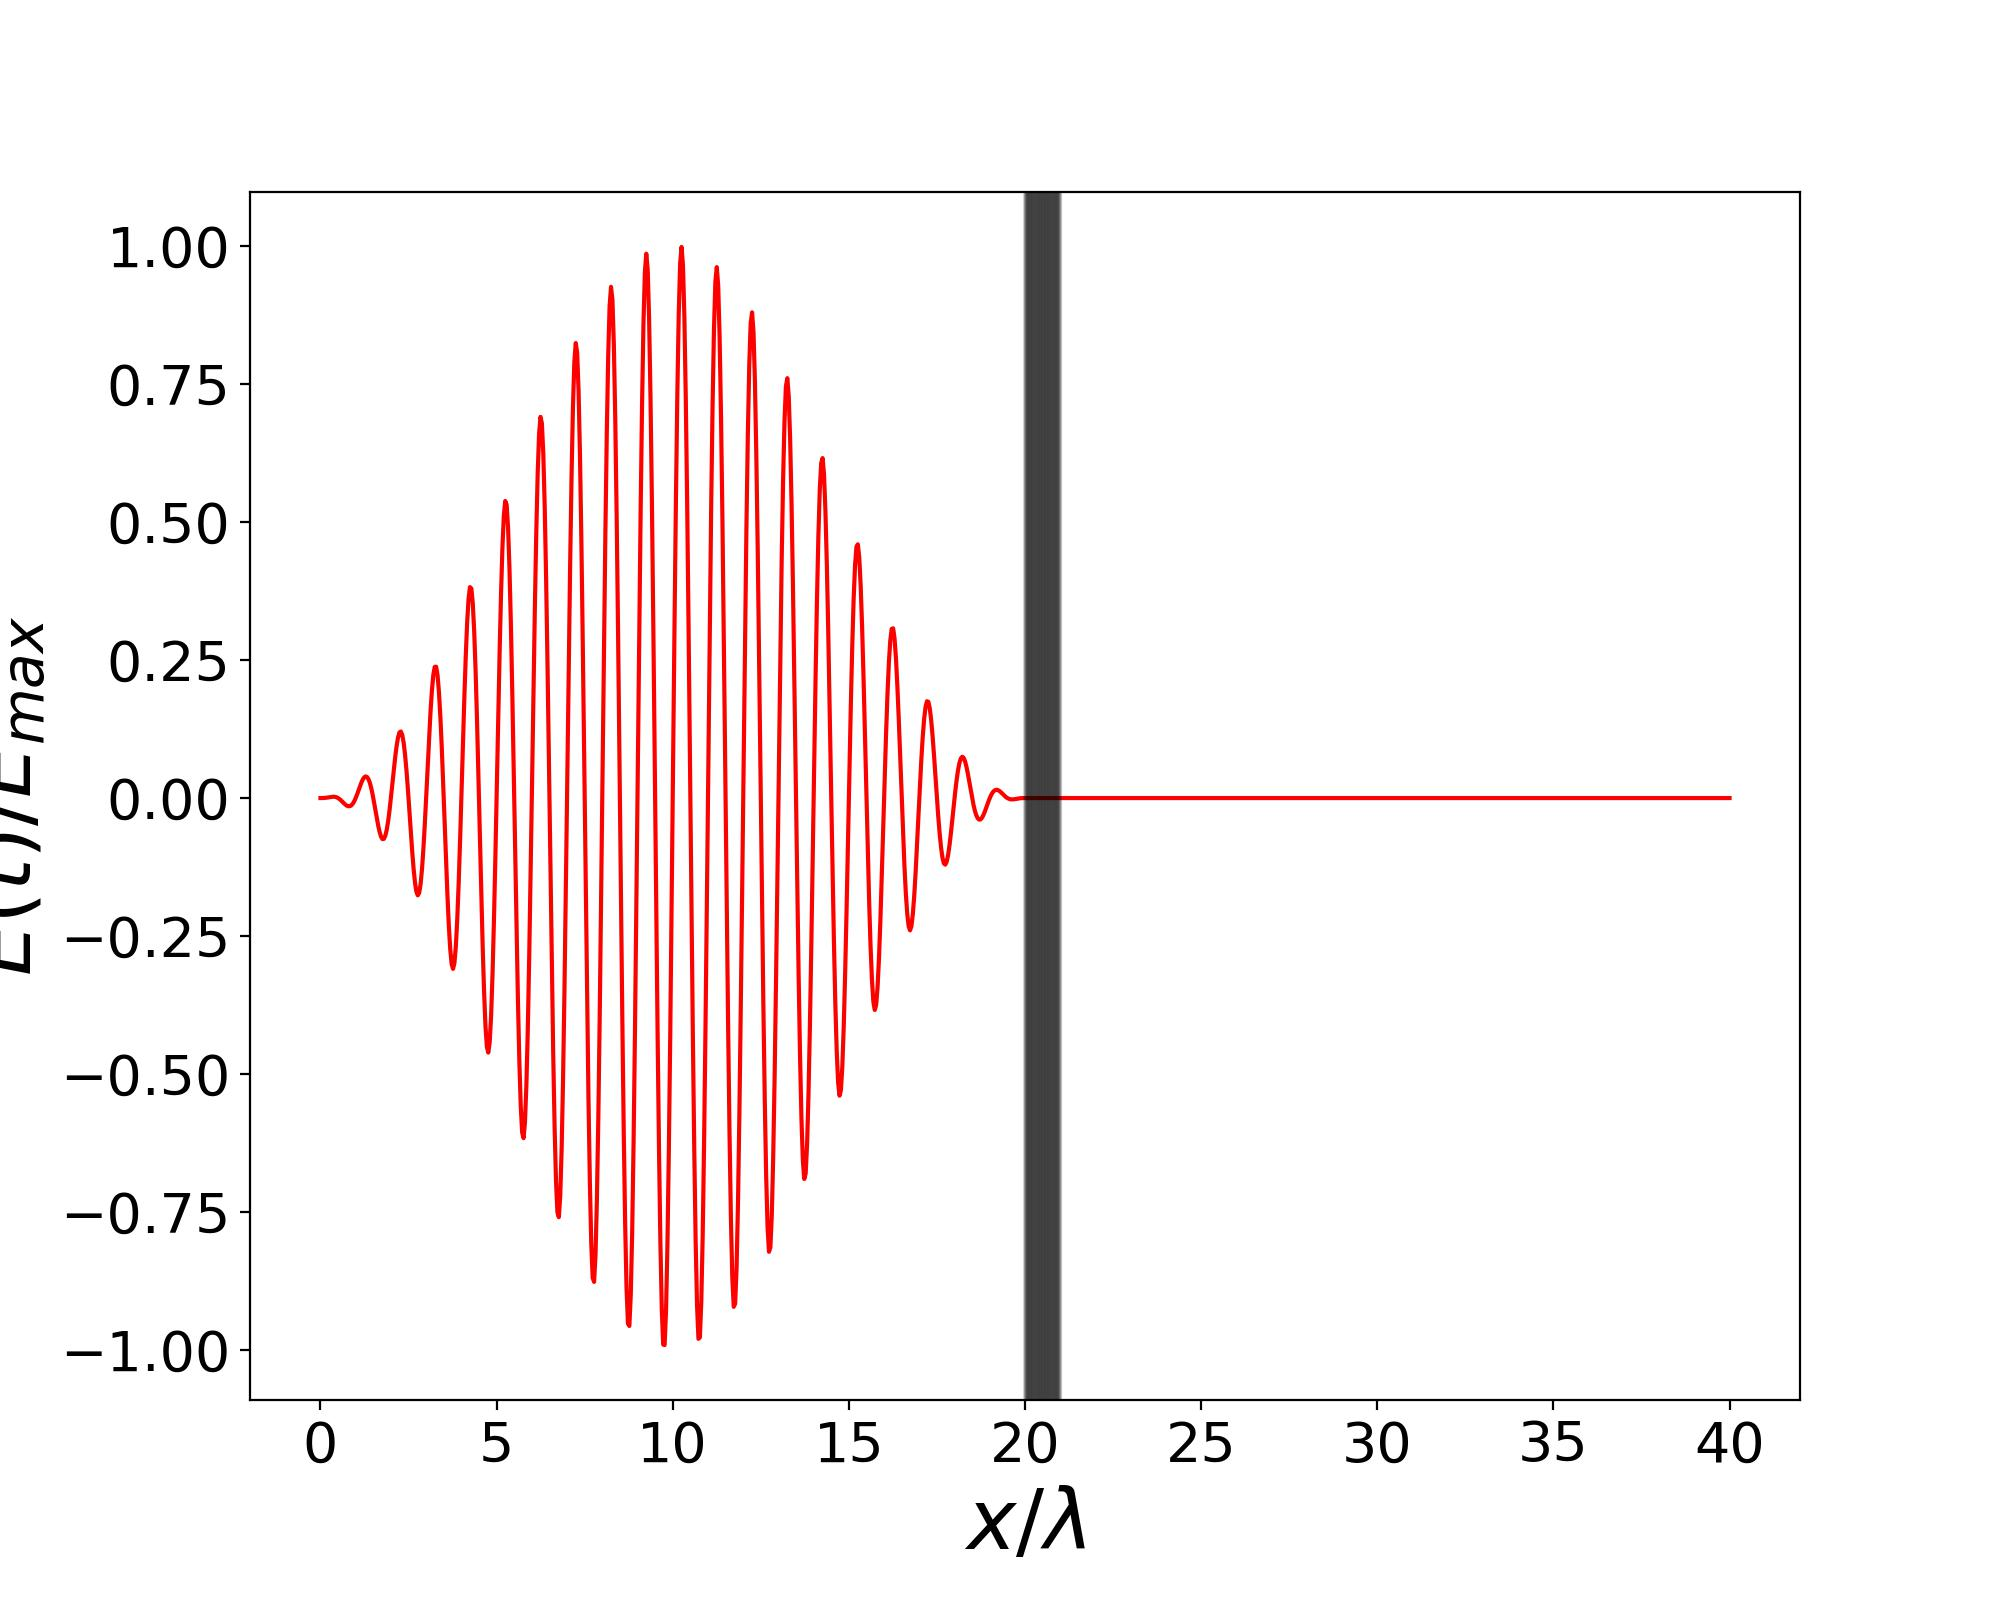
\includegraphics[width=0.9\textwidth, height=0.42\textheight]{images/field.jpg}
        \label{fig:field}
    \end{minipage}
    \begin{minipage}[h]{0.48\linewidth}
        \begin{figure}
            \centering
            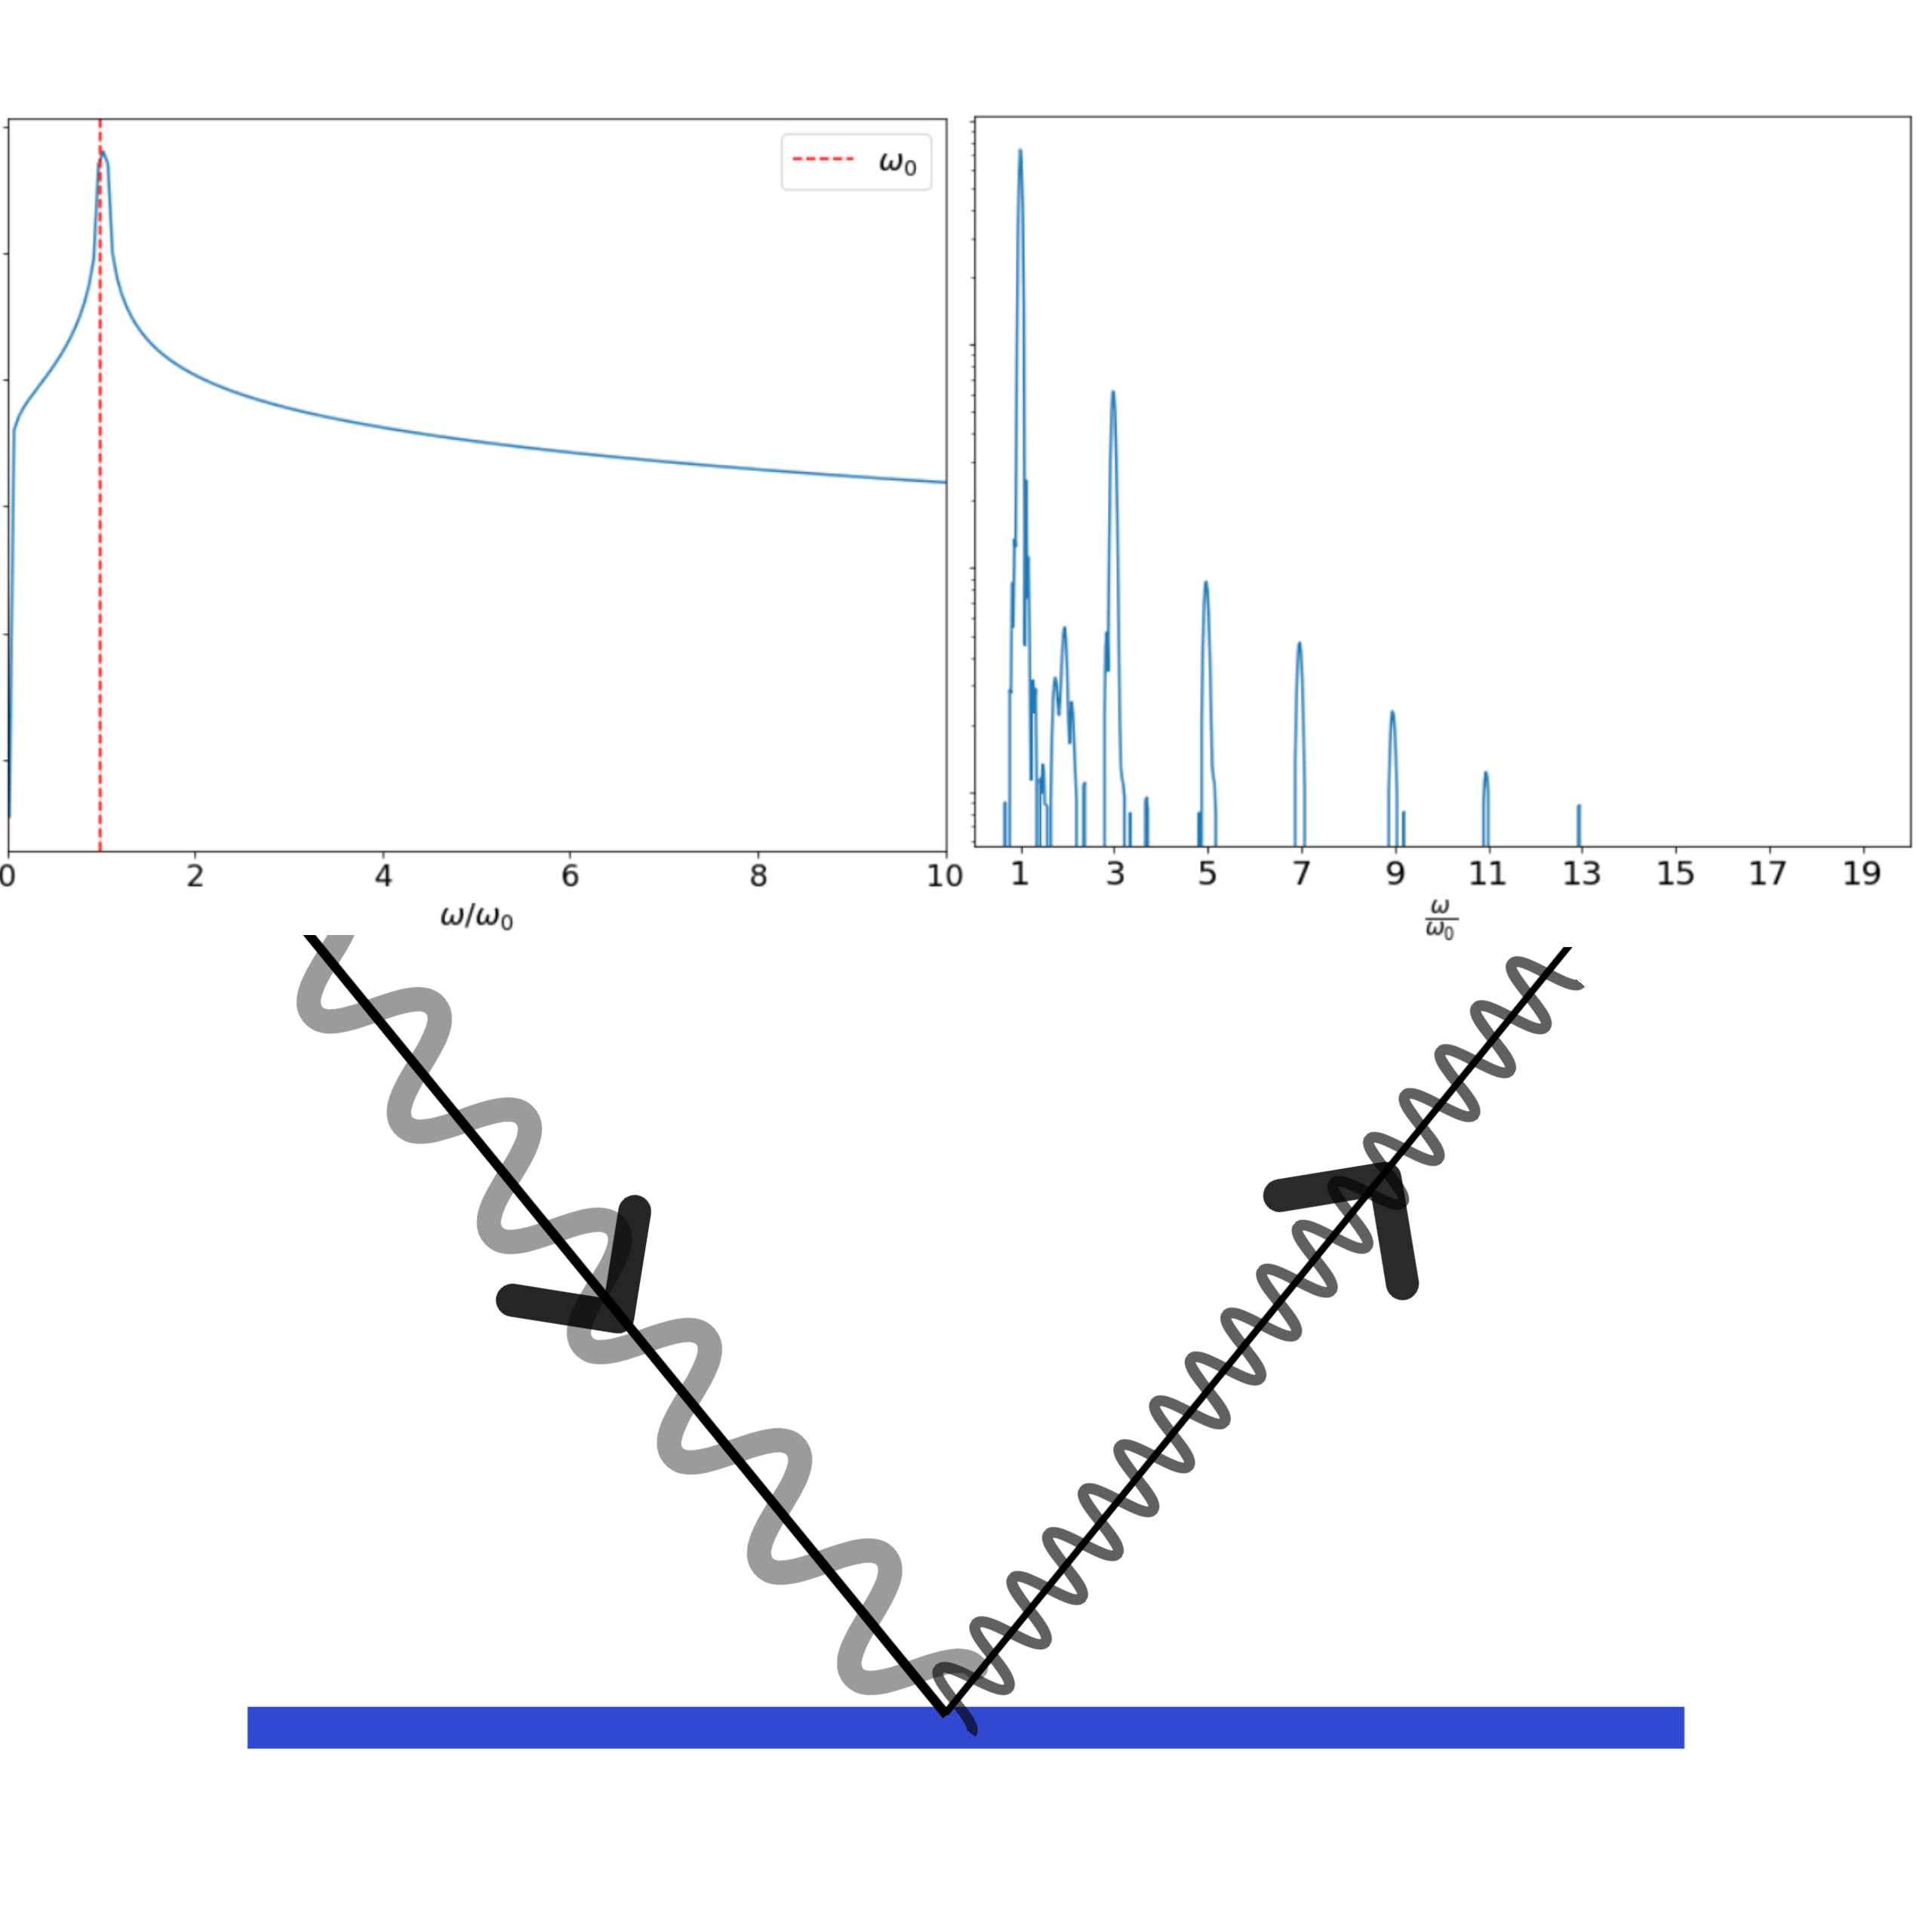
\includegraphics[width=0.9\textwidth, height=0.42\textheight]{images/harmonics.png}
            \label{fig:harmonics}
        \end{figure}
    \end{minipage}
\end{frame}

\begin{frame}
    \frametitle{Summary of Work Done in Previous Semester}
    \small
    \begin{itemize}
        \item Interaction of highly intense laser pulse with overdense and underdense plasma
        \item Change in effective critical density of plasma for relativistic laser pulse
        \item The oscillations of plasma surface.
              \begin{itemize}
                  \item Oscillations increases with increase in intensity
                  \item Surface oscillations have even harmonics
              \end{itemize}
        \item Study of high harmonics generation in laser plasma interaction (normal incidence)
              \begin{itemize}
                  \item Only odd harmonics are generated
                  \item A resonance at $n_0/n_c=4$ is also observed
                  \item Increasing intensity and pulse duration increases number of harmonics
                  \item No effect of the envelopes
              \end{itemize}
    \end{itemize}

    \textbf{What Now?}
    \begin{itemize}
        % \item A brief overview of theory related to High Harmonic Generation (HHG)
        \item Effect of Super Gaussian (SG) envelopes on the generated high harmonics
        \item Oblique incident and p- and s-polarized laser
        \item Selection rule for p- and s-polarized laser
    \end{itemize}
\end{frame}

% \begin{frame}
%     \frametitle{PIC Cycle}
%     \small
%     The simulation uses \textit{EPOCH}\footnotemark  which implements a particle in cell algorithm.
%     \begin{figure}
%         \centering
%         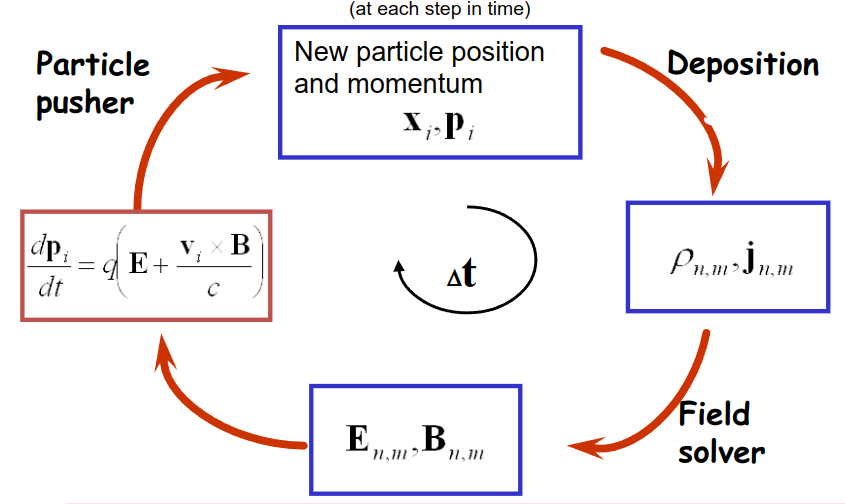
\includegraphics[width=0.9\textwidth, height=0.60\textheight]{images/PIC.png}
%         \label{fig:pic}
%     \end{figure}
%     \begin{itemize}
%         \item Interaction of laser pulse with plasma
%         \item Effect of relativistic laser pulse
%     \end{itemize}
%     \footnotetext[4]{\textit{T D Arber et al} 10.1088/0741-
%         3335/57/11/113001}
% \end{frame}
\begin{frame}
    \frametitle{Simulation Details}
    \small
    We want to study the effect of super Gaussian envelope on the generated high harmonics. We performed some simulations in 1D3V. Here are some parameters:

    \begin{minipage}[t]{0.48\linewidth}
        % left particle
        \begin{itemize}
            \item Particles per cell: 100
            \item Number of cells: 16000
            \item Pulse duration $= 20 \tau$ ($\tau\approx 3.3 fs$)
            \item Simulation time $= 40 \tau$
            \item Wavelength $\lambda_l = 1 \mu m$
            \item Intensity of laser for $a_0 = 1$ is $I = 1.37 \times 10^{18} W/cm^2$
        \end{itemize}
        We also performed simulations with p- and s-polarized laser incidence at oblique angle.
    \end{minipage}
    \begin{minipage}[t]{0.48\linewidth}
        \begin{figure}
            \centering
            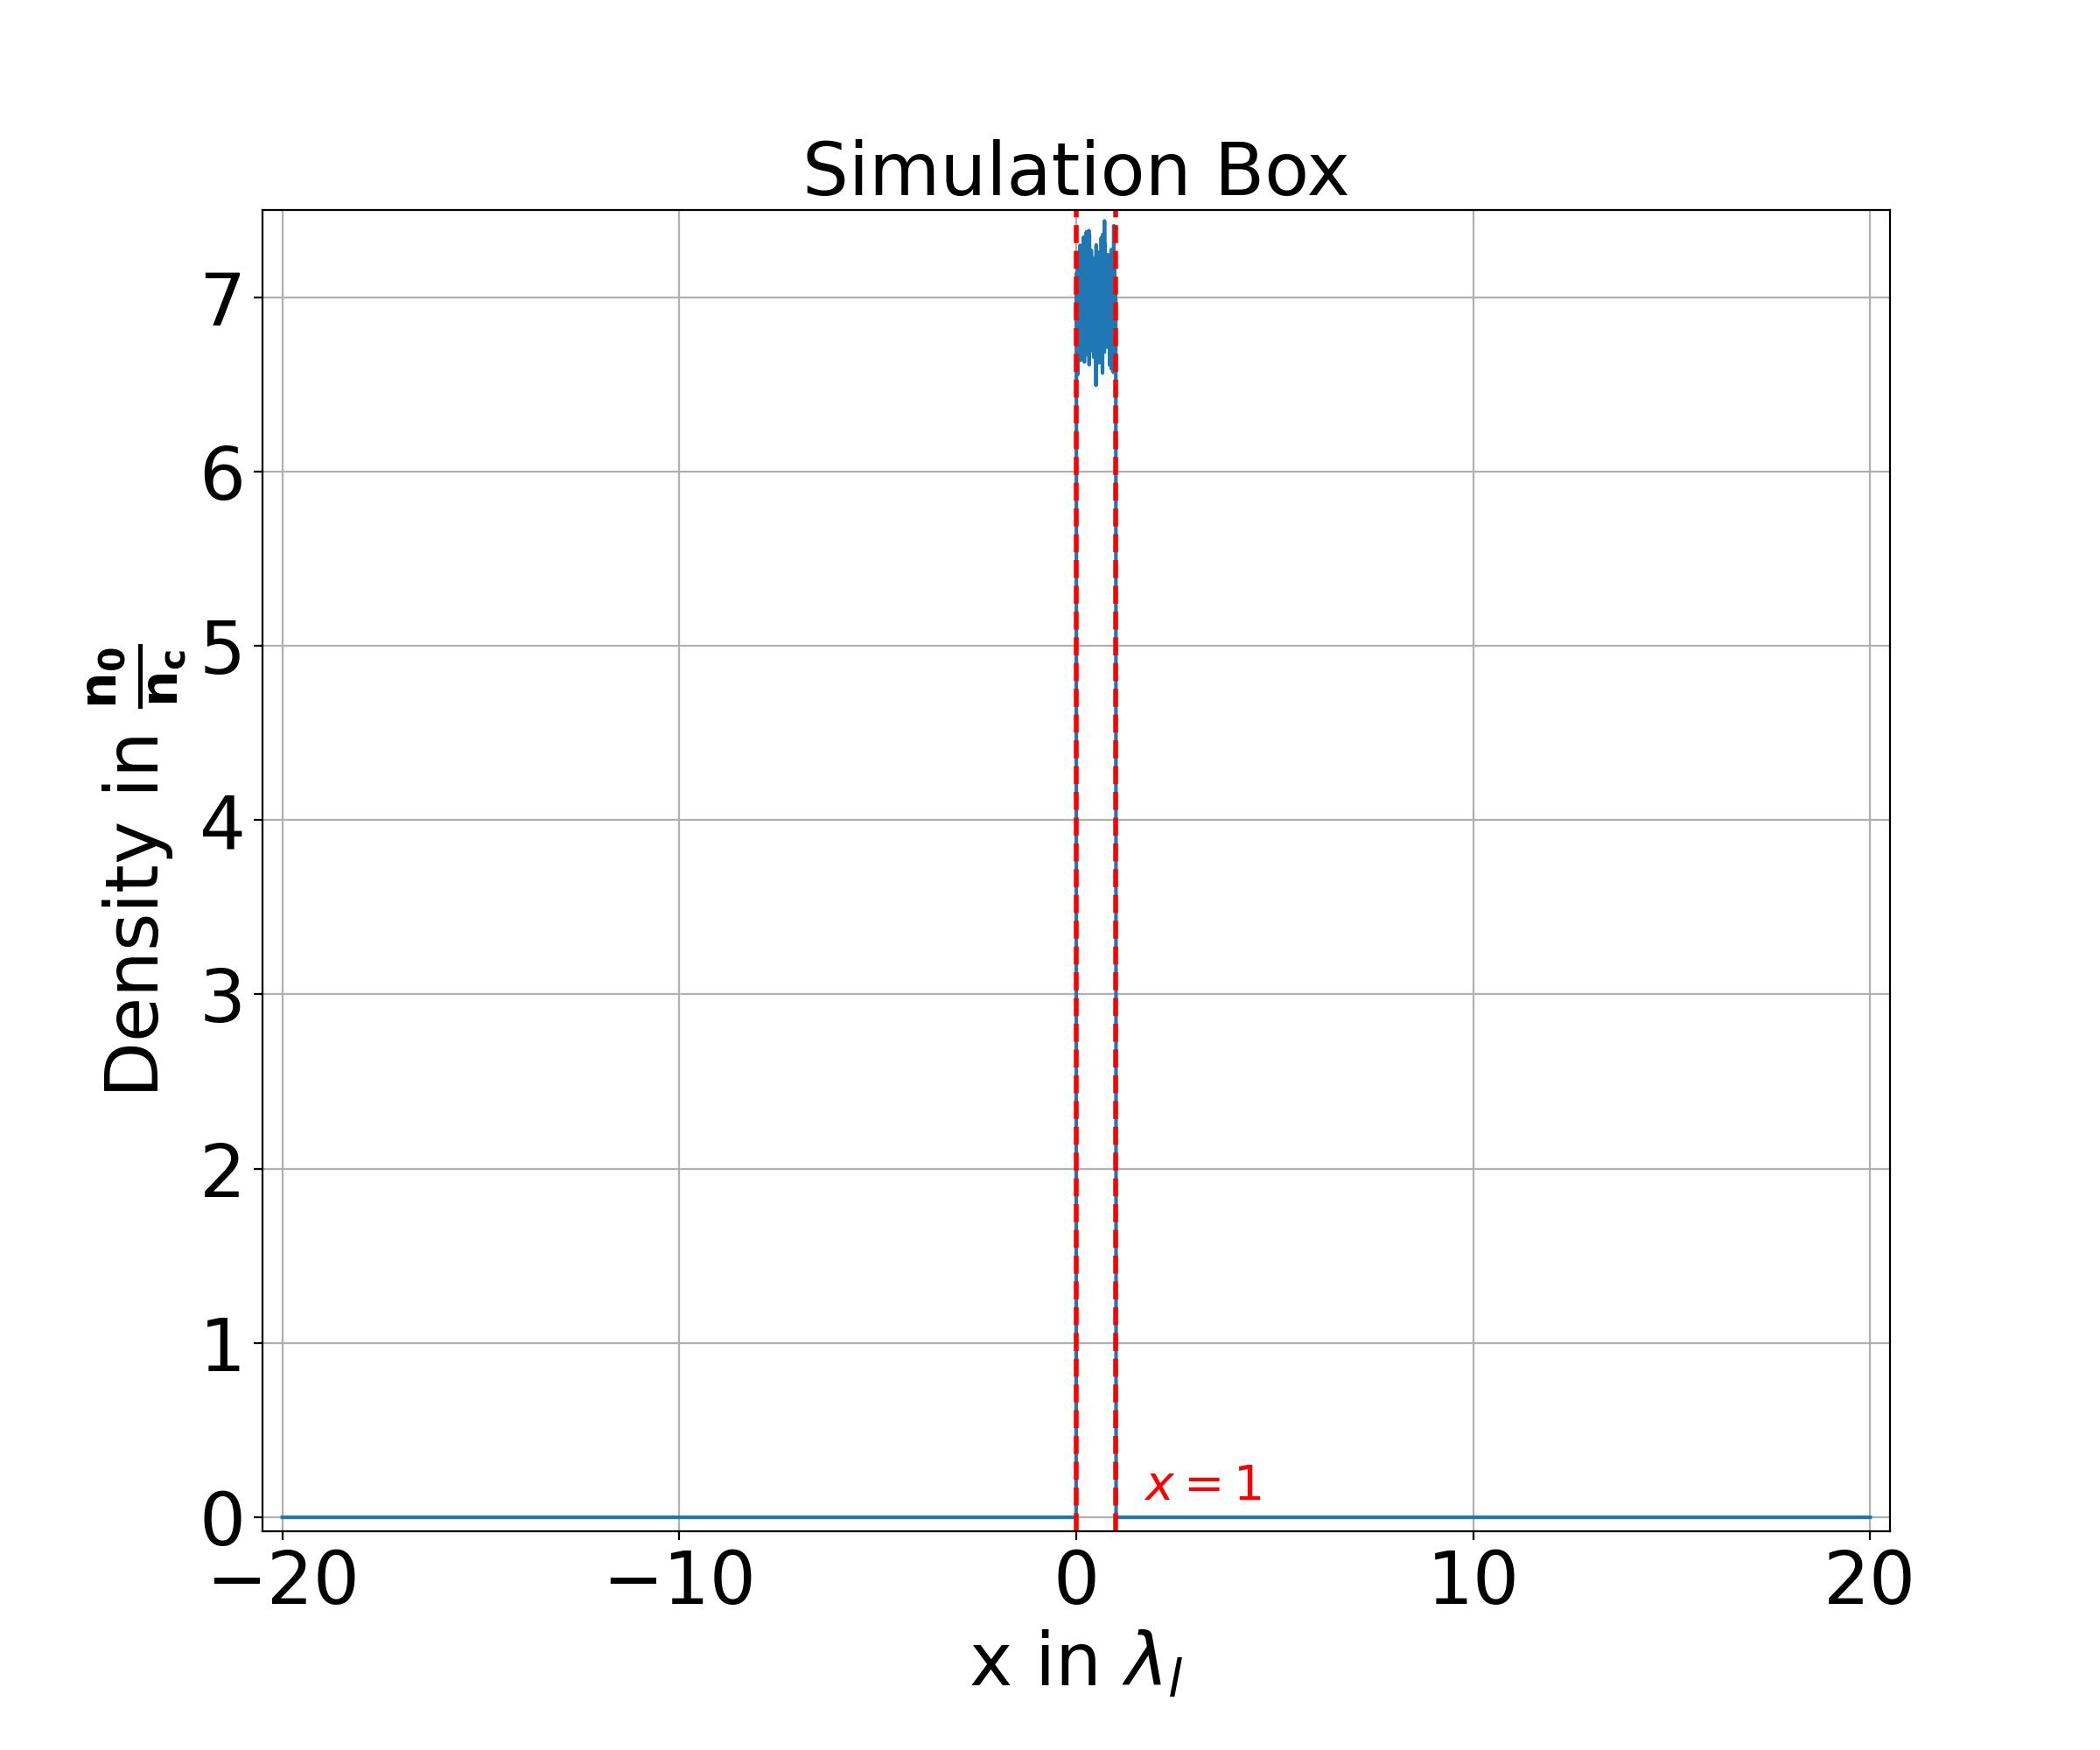
\includegraphics[width=1.0\textwidth, height=0.62\textheight]{images/plasma.jpg}
            \label{fig:plasma}
        \end{figure}
    \end{minipage}
\end{frame}

\begin{frame}
    \frametitle{Oblique Incidence: Transformations}
    \small
    \begin{itemize}
        \item We follow Bourdier\footnote{\textit{Bourdier,A. } 10 . 1063 / 1.864355} to make a transformation which lets us simulate oblique incidence in 1D.
    \end{itemize}
    \begin{minipage}[t]{0.35\linewidth}
        % \tiny
        \begin{align*}
            \begin{split}
                &\text{For p-polarization}\\
                \mathbf{E}_L  & = E_0(-\sin\alpha \hat{x} + \cos\alpha \hat{y}) \\
                \mathbf{E}_M  & = E_0\cos\alpha \hat{y}                         \\
                c\mathbf{B}_L & = E_0\hat{z}                                    \\
                c\mathbf{B}_M & = E_0\cos\alpha \hat{z}\\
                &\text{For s-polarization}\\
                \mathbf{E}_L & = E_0\hat{z}                                    \\
                \mathbf{E}_M & = E_0\cos\alpha \hat{z}                        \\
                c\mathbf{B}_L & = E_0(\sin\alpha \hat{x} - \cos\alpha \hat{y}) \\
                c\mathbf{B}_M & = -E_0\cos\alpha \hat{y}
            \end{split}
        \end{align*}

    \end{minipage}
    \begin{minipage}[t]{0.60\linewidth}
        \begin{figure}
            \centering
            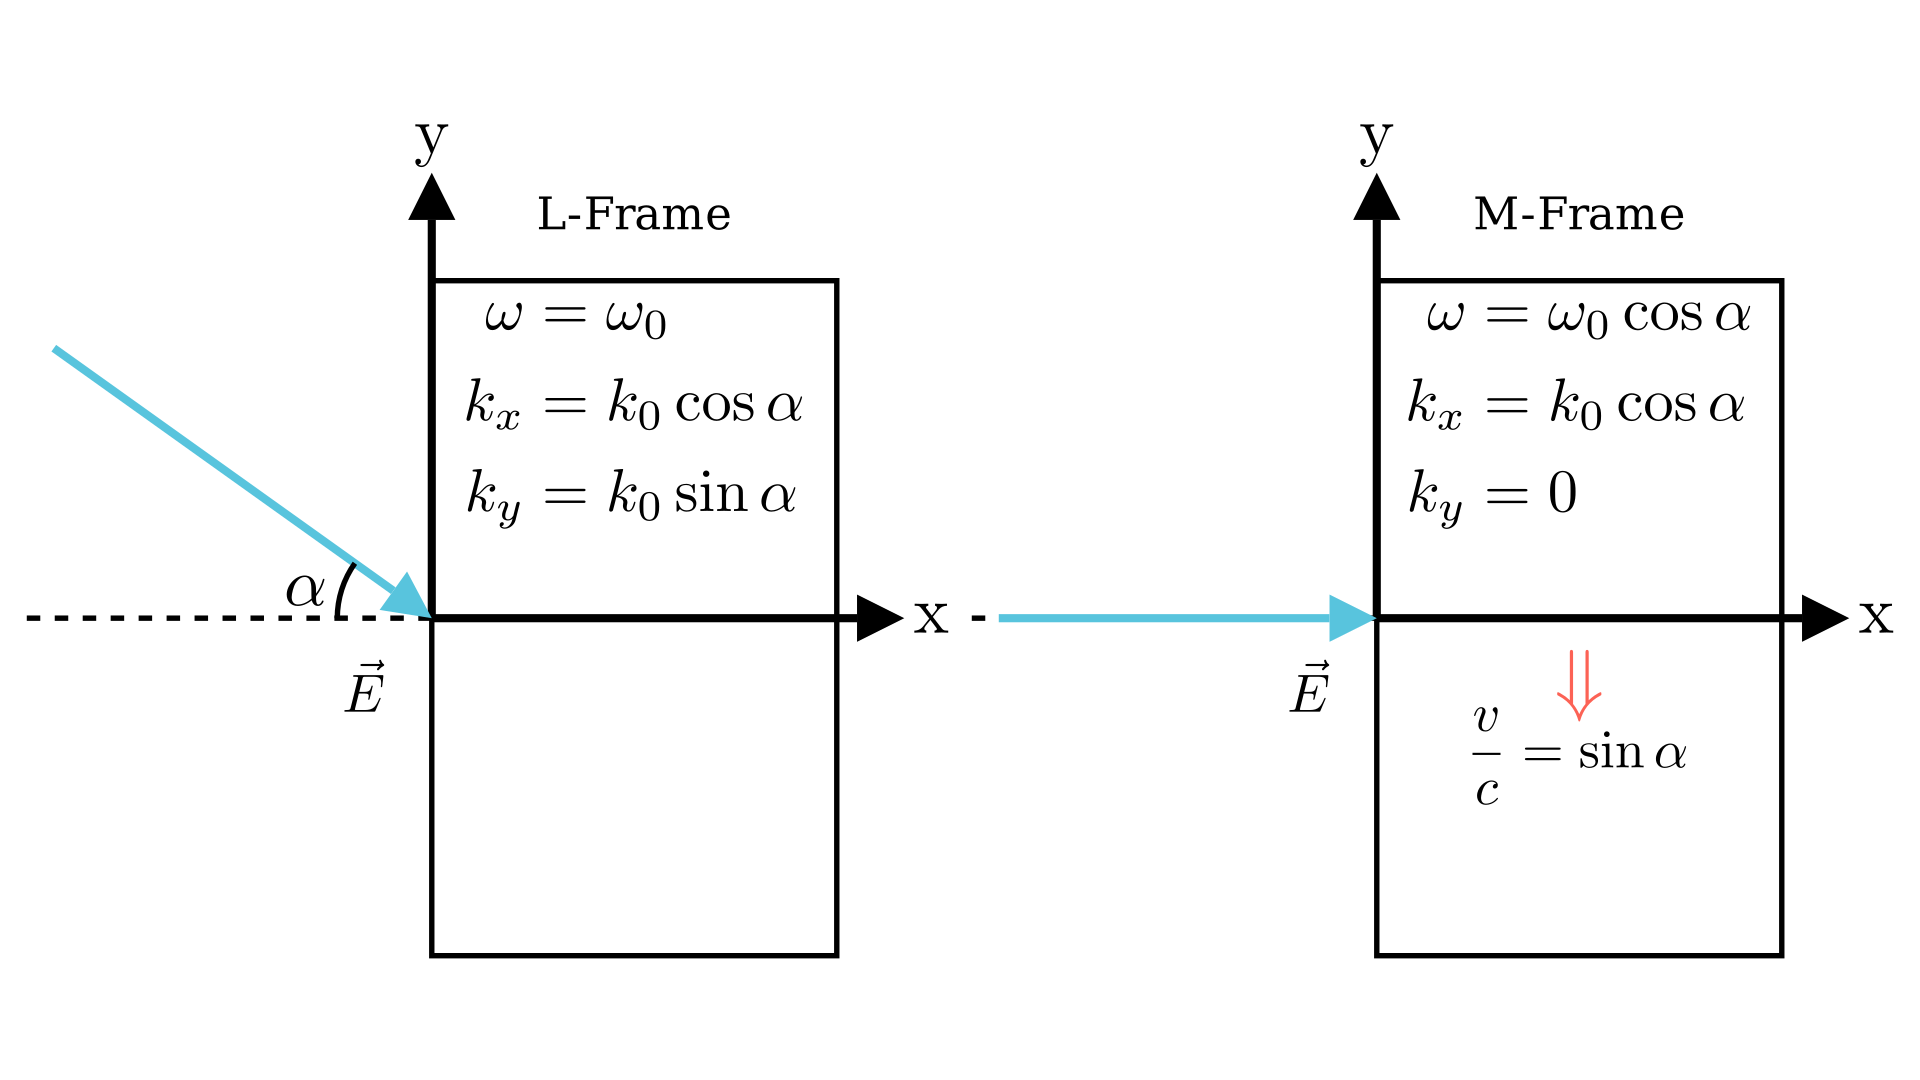
\includegraphics[width=1.0\textwidth, height=0.62\textheight]{images/frames.png}
            \label{fig:frames}
        \end{figure}
    \end{minipage}
\end{frame}

\begin{frame}
    \frametitle{p- and s- Polarized Laser: Selection Rule}
    \begin{minipage}[h]{0.18\linewidth}
        \small{p-Polarization}
        \tiny{
            \textbf{p-Polarized:} None

            \textbf{s-Polarized:} Odd, Even}
    \end{minipage}
    \begin{minipage}[h]{0.8\linewidth}
        \centering
        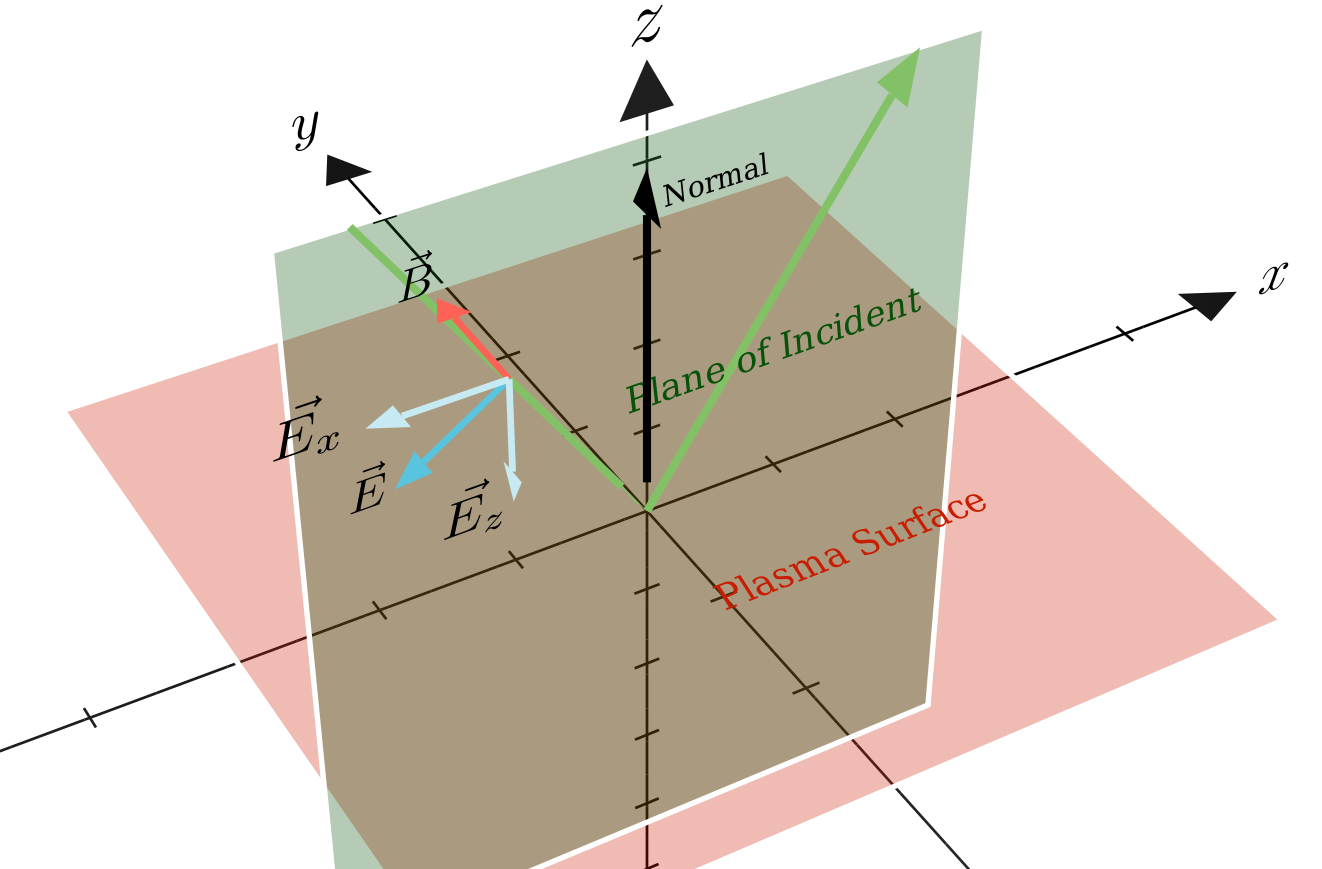
\includegraphics[width=0.9\textwidth, height=0.42\textheight]{images/p.png}
        \label{fig:p}
    \end{minipage}

    \begin{minipage}[h]{0.8\linewidth}
        \centering
        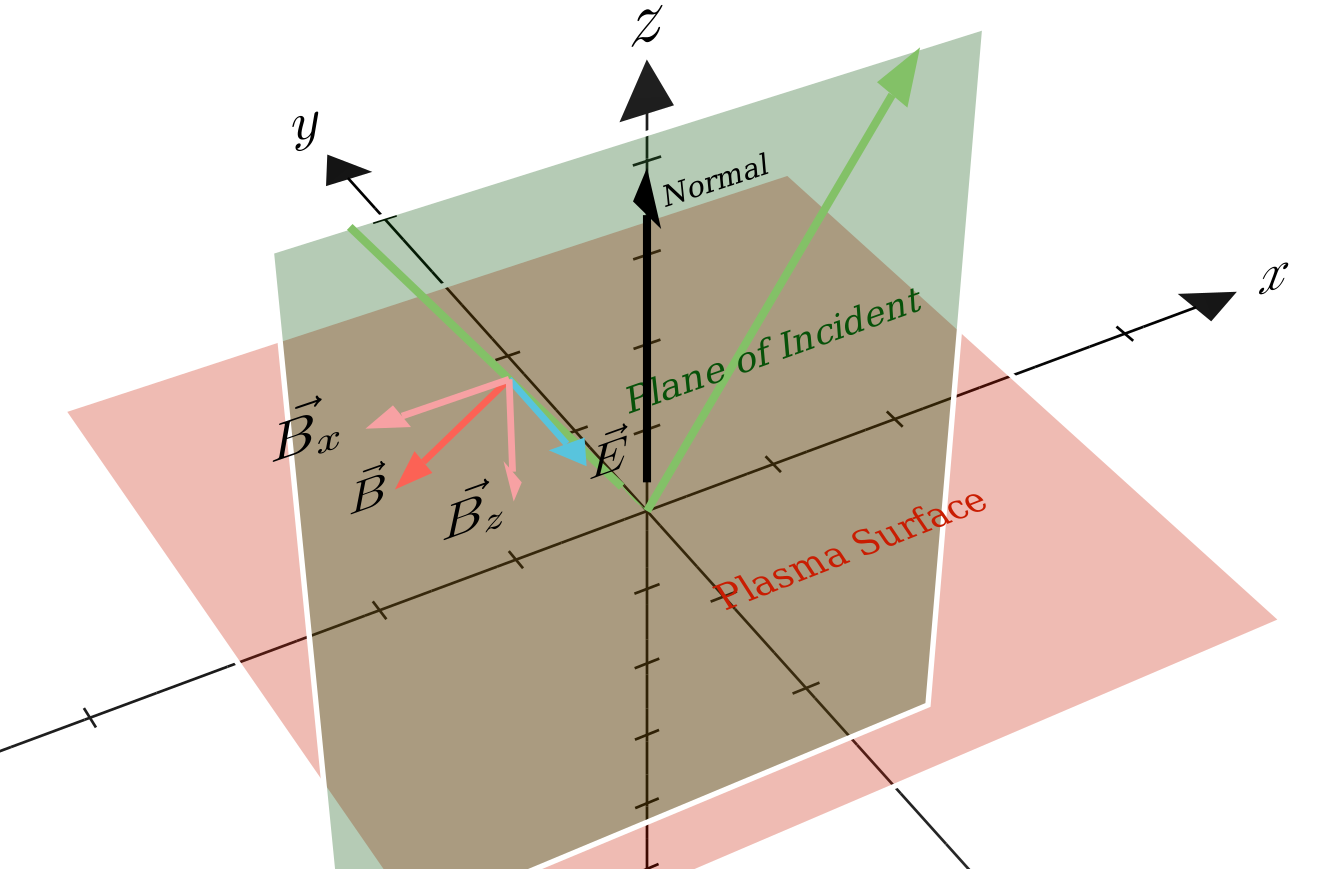
\includegraphics[width=0.9\textwidth, height=0.42\textheight]{images/s.png}
        \label{fig:s}
    \end{minipage}
    \begin{minipage}[h]{0.18\linewidth}
        \small{s-Polarization}
        \tiny{
            \textbf{p-Polarized:} Even

            \textbf{s-Polarized:} Odd}
    \end{minipage}

\end{frame}

\begin{frame}
    \frametitle{Results: SG Envelope}
    \begin{figure}[h]
        \centering
        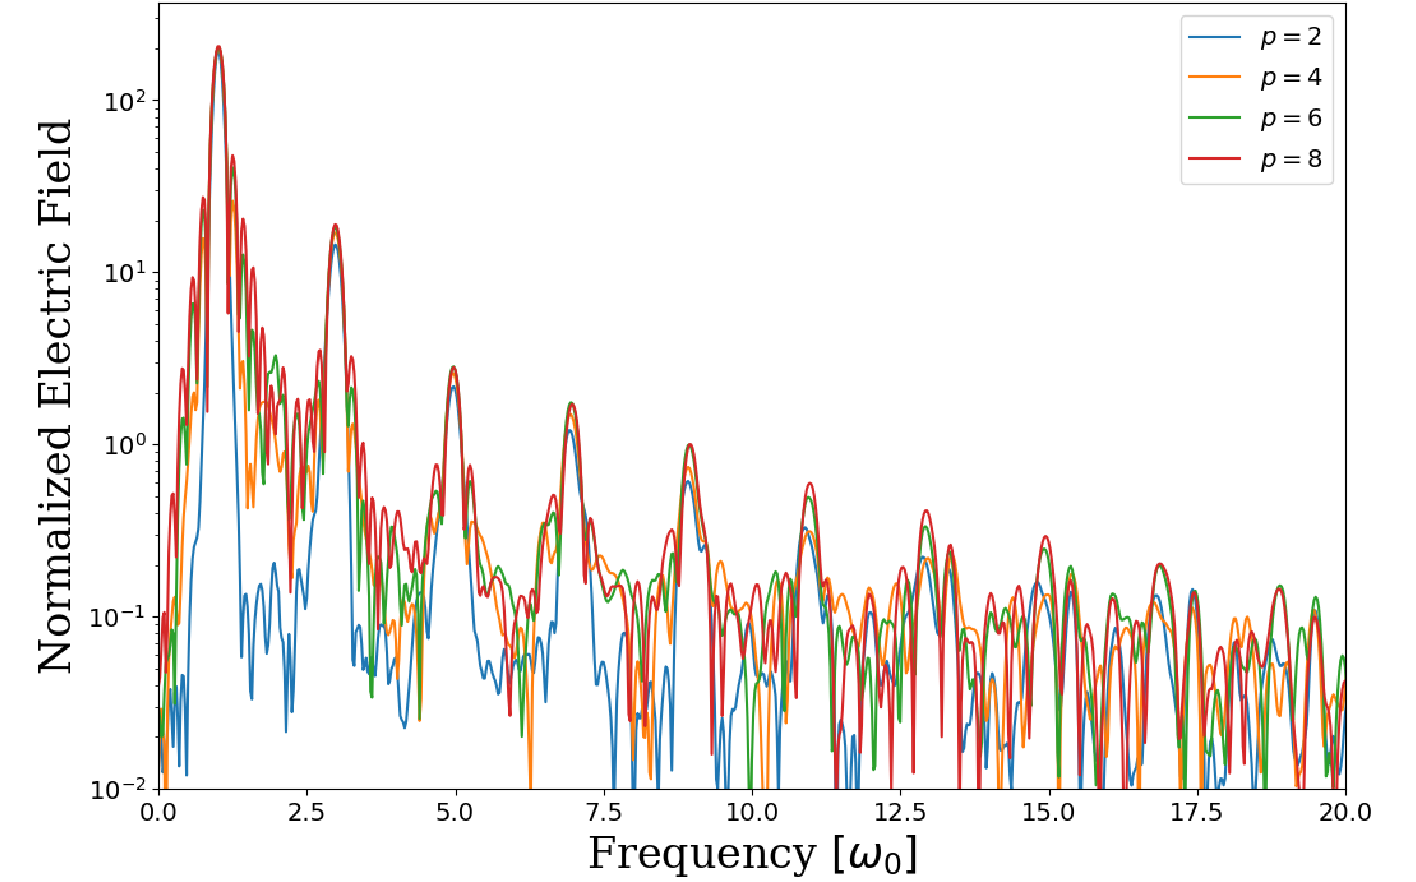
\includegraphics[width=0.85\textwidth]{images/sg_2.png}
        \caption{The spectrum of SG envelopes with power 2,4,6, and 8 is shown in a sigle plot. A small increase in the peak amplitude is observed with increasing power.}
        \label{fig:sg}
    \end{figure}
\end{frame}

\begin{frame}
    % \begin{table}[h]
    %     \tiny
    %     \centering
    %     \vspace{0.5cm}
    %     \label{tab:selection-rule}
    %     \begin{tabular}{|l|l|l|}
    %         \hline
    %                                          & \textbf{s-polarized Harmonics} & \textbf{p-polarized Harmonics} \\ \hline
    %         \textbf{s-Polarized Fundamental} & Odd                            & Even                           \\ \hline
    %         \textbf{p-Polarized Fundamental} & None                           & Odd and Even                   \\ \hline
    %     \end{tabular}
    % \end{table}
    \frametitle{Results: p-Polarized Laser}
    \begin{figure}[h]
        \centering
        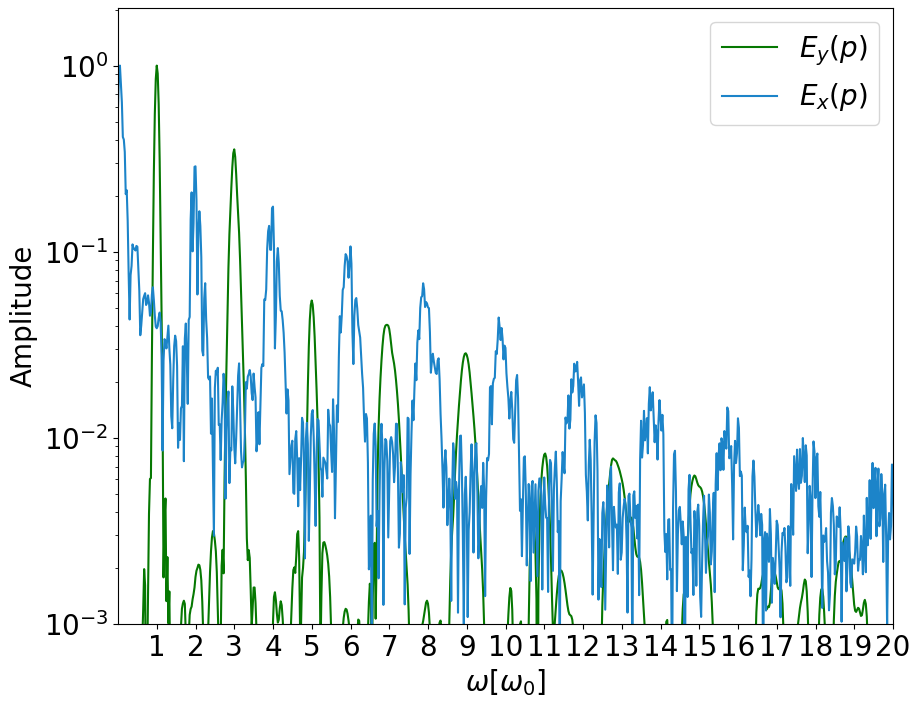
\includegraphics[width=0.75\textwidth]{images/p_fft.png}
        \caption{\small{Spectrum of HHG for p-polarized light. Simulation parameters are $\alpha = \pi/6$, the denity is $n_0 = 7n_c$ and $a_0 = 4$}}
    \end{figure}
\end{frame}

\begin{frame}
    \frametitle{Results: s-Polarized Laser}
    \begin{figure}
        \centering
        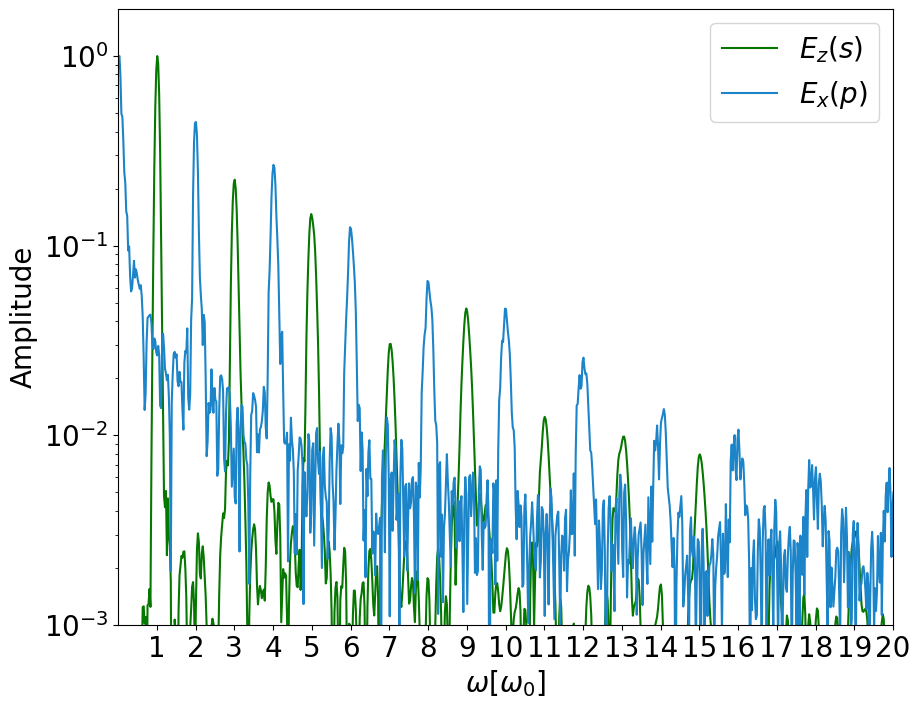
\includegraphics[width=0.75\textwidth]{images/s_fft.png}
        \caption{\small{Spectrum of HHG for s-polarized light. Simulation parameters are $\alpha = \pi/4$, the denity is $n_0 = 7n_c$ and $a_0 = 4$}}
    \end{figure}
\end{frame}

\begin{frame}
    \frametitle{Current Status and Future Plan of Work}
    \small
    \textbf{Current Status}
    \begin{itemize}
        \item A brief overview of HHG generation in laser plasma interaction
        \item SG envelopes has very little effect on the generated harmonics
        \item For p-polarized laser, even and odd p-polarized harmonics.
        \item For s-polarized laser, odd s-polarized hyarmonics and even p-polarized harmonics.
    \end{itemize}
    \textbf{Future Plan of Work}
    \begin{itemize}
        \item Study oblique incidence and polarization more regously.
        \item Do 2D simulations.
        \item Compare it with the 1D results.
    \end{itemize}
    \textbf{Acknowledgement}

    We would like to extend our sincerest gratitude to Professor Vikrant Saxena for his unwavering support, patience, motivation, enthusiasm, and invaluable guidance.
\end{frame}
\end{document}